\documentclass[a4paper,12pt]{article}

% Paquetes básicos
\usepackage[utf8]{inputenc}
\usepackage[T1]{fontenc}
\usepackage[spanish]{babel}
\usepackage{graphicx}
\usepackage{xcolor}
\usepackage{lipsum}
\usepackage{geometry}
\geometry{top=3cm, bottom=3cm, left=2.5cm, right=2.5cm}

% Paquetes para diseño
\usepackage{titlesec}
\usepackage{fancyhdr}
\usepackage{amsmath}
\usepackage{amssymb}
\usepackage{hyperref}
\usepackage{float}

% Paquetes para el entorno lstlisting
\usepackage{listings}
\usepackage{inconsolata}

% Paquete para diagramas
\usepackage{tikz}
\usetikzlibrary{shapes, arrows.meta, positioning}

% Paquete para fondo
\usepackage{background}

% Configuración de lstlisting
\lstset{
    language=Python,
    basicstyle=\ttfamily\small,
    keywordstyle=\color{blue}\bfseries,
    stringstyle=\color{teal},
    commentstyle=\color{gray}\itshape,
    numbers=left,
    numberstyle=\tiny\color{gray},
    backgroundcolor=\color{black!5},
    frame=single,
    rulecolor=\color{black!50},
    breaklines=true,
    captionpos=b,
    showstringspaces=false
}


%comandos
\usepackage{amsmath}
\newcommand{\flechita}{$\rightarrow$}

% Configuración de título
\titleformat{\section}{\normalfont\Large\bfseries}{\thesection}{1em}{}

% Información del documento
\title{
    \vspace{-2cm}
    
\includegraphics[width=0.3\textwidth]{images/fccee.jpg} \\ % Cambia el logo si es necesario
    \LARGE Ingeniería Informática + ADE\\
    \large Universidad de Granada (UGR)\\[1cm]
}
\author{\textbf{Autor:} Ismael Sallami Moreno}
\date{\textbf{Asignatura:} Resúmenes de Contabilidad Financiera I Tema 2: Existencias: Compras y Ventas}

% Configuración del fondo
\backgroundsetup{
    scale=1,
    color=black,
    opacity=0.2,
    angle=0,
    position=current page.south,
    vshift=0pt,
    hshift=0pt,
    contents={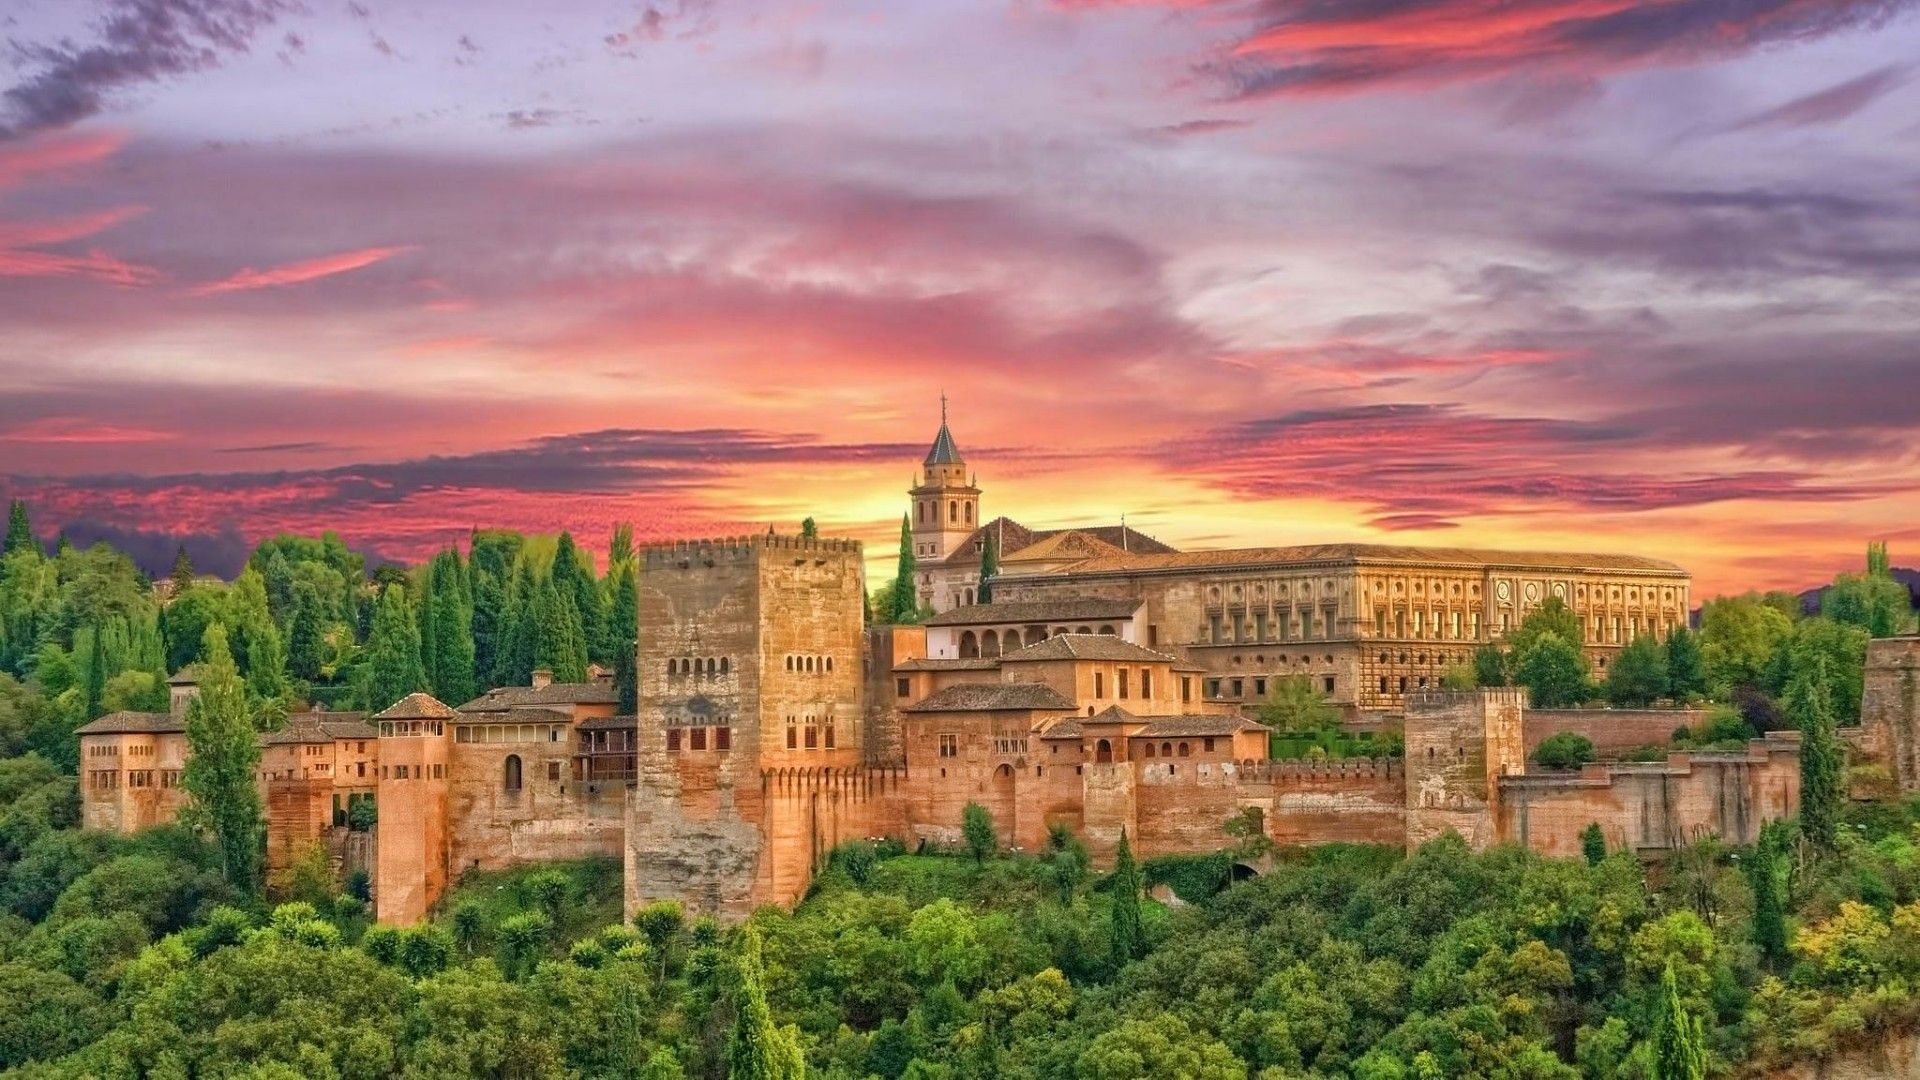
\includegraphics[width=\paperwidth,height=\paperheight,keepaspectratio]{images/granada.jpg}}
}

% Configuración del encabezado y pie de página
\usepackage{times}
\pagestyle{fancy}
\fancyhf{}
\fancyhead[L]{\textbf{\textsf{\leftmark}}}
\fancyhead[R]{\textbf{\textsf{\thepage}}}
\fancyfoot[C]{\thepage}

% Inicio del documento
\begin{document}

% Portada
\maketitle
\thispagestyle{empty}

\begin{center}
    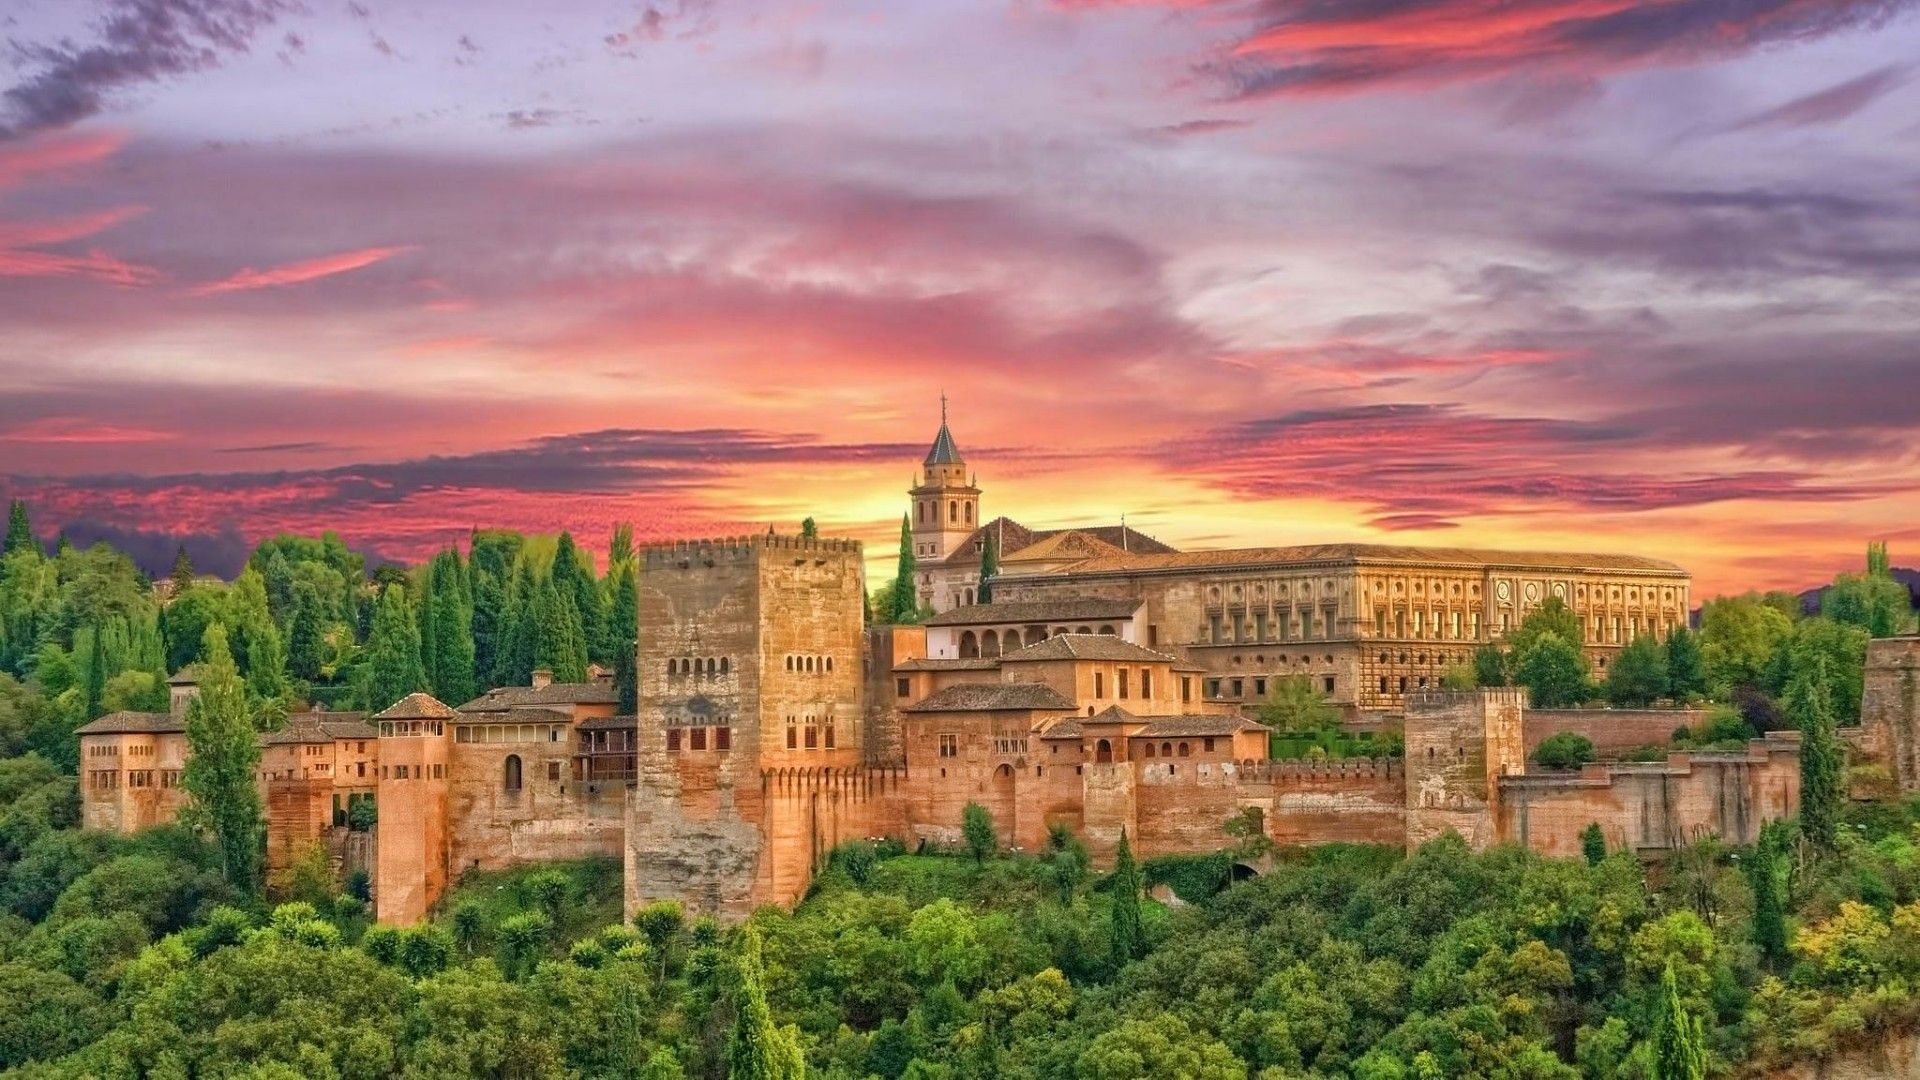
\includegraphics[width=\textwidth,height=0.4\textheight,keepaspectratio]{images/granada.jpg} \\ % Añade tu imagen de fondo
    \vfill
\end{center}

\newpage

% Índice (opcional)
\tableofcontents
\newpage





\section{Existencias: Concepto, características y tipología}

Las existencias son activos que son poseídos para su venta en operaciones de explotación, incorporarse al proceso productivo, se consumidos en el proceso de producción o bien para la prestación de servicios.\\\\
Tipos de existencias según el destino de las mismas:
\begin{itemize}
    \item Activos poseídos para su venta sin transformación (Cuentas: 30,31 320, 321, 322, 325, 326, 327, 328)
    \item Activos poseídos para su venta con transformación posterior (Cuentas: 33, 34, 35, 360, 365 y 368)
    \item Activos poseídos para utilizar en cualquier fase del proceso de transformación de bienes y servicios
\end{itemize}
\textit{Mirar páginas 54 y 55 del manual}

\section{Reconociminento y valoración de las existencias}

\subsection{Valoración de las entradas de las existencias}

Los que son adquiridos del exterior serán valorados a su precio de coste, mientras que los que son producidos por la empresa se valorarán a su coste de producción.

\subsubsection{Precio de adquisición de las existencias}

Esta formado por el precio del proveedor más los gastos adicionales para que se encuentren en el lugar adecuado para la venta, como transportes, seguros, impuestos, etc. Los impuestos indirectos que gravan las existencias solo serán incluidos en el precio de adquisición si no son recuperables.


\begin{table}[H]
    \begin{tabular}{|p{5cm}|p{5cm}|}
    \hline
    \textbf{PRECIO DE COMPRA [FACTURA]} & \textbf{GASTOS ADICIONALES} \\ \hline
    \begin{itemize}
        \item Importe facturado
        \item (-) Descuentos y rebajas
        \item (+) Impuestos no repercutibles (NV.10.1) no recuperable
        \item (+) Gastos financieros si condiciones de funcionamiento más de 1 año (NV. 1)
        \item (-) Intereses incorporados a los débitos
        \item (+) Intereses incorporados a los débitos si se cumple lo siguiente (NV. 9 y 10.1):
        \begin{itemize}
            \item Vto. no superior al año,
            \item No tienen interés contractual.
            \item Actualización no significativa
        \end{itemize}
    \end{itemize} & 
    \begin{itemize}
        \item Transporte.
        \item Aranceles y otros impuestos no repercutibles.
        \item Seguros de transporte.
        \item Conservación, inspección y depósito en tránsito.
    \end{itemize} 
    Hasta que los bienes se hallen ubicados para su venta 
    \\ \hline
    \end{tabular}
\end{table} 
    
\subsubsection{Coste de producción de las existencias}

Se añade el precio de adquisición de las materias primas, los gastos de producción y los gastos generales de fabricación.


\subsection{Métodos de asignación de valor}
Depende de si los bienes son intercambialaes o no. Cuando se trate de no intercambiable el valor que se asignará indentificando el precio y los costes específicamente imputables a cada bien indidualmente. Si son bienes intercambiables podrá adoptarse métodos como el método FIFO o el PMP(Precio Medio Ponderado). Únicamente se usará un método para cumplir con el principio de uniformidad.

\subsubsection{PMP (Precio Medio Ponderado)}

Siendo $Q_{i}$ la cantidad de existencias adquiridas a un precio $P_{i}$, el precio medio ponderado se calcula como:
\[
    PMP = \frac{\sum_{i=1}^{n}Q_{i}P_{i}}{\sum_{i=1}^{n}Q_{i}}
\]

\subsubsection{FIFO (First In, First Out)}

Se considera que las primeras existencias adquiridas son las primeras que se venden. Se calcula el coste de las existencias finales a partir de las primeras adquiridas.

\section{Valoración Posterior de las Existencias}

Tenemos que tener en cuenta la depreciación de valor:
\begin{itemize}
    \item Deterioro de valor: Debemos de tener en cuenta el principio de prudencia, por lo que se considerará pérdidas del ejercicios apareciendo en la cuenta de Pérdidas y Ganancias por su importe corregido.
    \item Pérdida de valor: Deberá de considerarse al valorar las existencias finales, quedando reflejada la pérdida de valor de forma implícita en la valoración de las existencias.
\end{itemize}

\subsubsection*{Criterio del Valor Neto Realizable}

Se establece que cuando éste sea inferior a su precio de adquisición o a su coste de producción, se efectuarán las oportunas correciones valorativas reconociéndolas como pérdidas en la cuenta de Pérdidas y Ganancias.

\section{Procedimientos de Contabilizacón de las existencias}

Si la cuenta de mercaderías sigue un procedimiento especulativo quiere decir que se debe de anotar en el Haber las ventas (\textit{minorando de las existencias}), pero evaluadas a precios de venta, por lo que en el movimiento de la cuenta se incluye la pérdida o ganancia habidas.\\\\
El PGC usa el procedimiento especulativo desglosado. Se usarán cuentas diferentes a las propias de existencias y que recojan dichas operaciones. Las cuentas de existencias se limitarán a recoger las existencias iniciales al inicio del ejercicio y las finales al final del mismo, es decir, lo que se denomina \textit{Variación de existencias}.


\subsection{Tratamiento Contable de las compras}

Si se realiza una compra se debe de cargar en la cuenta \textit{600 compra de mercaderías} y abonar en la cuenta \textit{400 proveedores}. Si se realiza una compra de mercaderías con IVA se debe de cargar en la cuenta \textit{600 compra de mercaderías} y abonar en la cuenta \textit{400 proveedores} y en la cuenta \textit{472 Hacienda Pública, IVA soportado}. Si se realiza una devolución de mercaderías se debe de cargar en la cuenta \textit{400 proveedores} y abonar en la cuenta \textit{608 devolución por compras}. En el caso de que se realice un descuento por volumen de compras debemos de dar de baja a la cuenta de proveedores y dar de alta a la cuenta \textit{609 rappels por compras}. Y si es por pronto pago debemos de usar la cuenta \textit{606 descuento por pronto pago}.

\subsection{Tratamiento Contable de las ventas}

Una empresa reconcerá los ingresos cuando se produzca la transferencia del control de los bienes y servicios comprometidos con el cliente. La empresa para reconcer dicho momento considerará los siguientes criterios/indicadores:
\begin{itemize}
    \item El cliente asume los riesgos y beneficios significativos.
    \item La empresa ha transferido la posesión física del activo.
    \item El cliente ha recibido el acuerdo con las especificaciones contractuales.
    \item La empresa tiene un derecho de cobro al transferir el activo.
    \item El cliente tiene la propiedad del activo.
\end{itemize}

\textit{No formará parte de los ingresos los impuestos que gravan las operaciones de entrega de bienes o servicios, como el IVA.}\\\\
El precio de la transacción es aquel que se entiende como el importe de la contraprestación que la empresa espera recibir a cambio de la entrega de bienes o servicios, puede ser fija, varible o una combinación de ambas.\\\\
Cuando se producen devoluciones de ventas se hace uso de una nueva cuenta que es la \textit{708 devoluciones de ventas}. Tiene naturaleza deudora y actuará como una cuenta compensadora de ingresos para la empresa.\\\\
Si la suma de precios de venta independientes supera la contraprestación acordada, la empresa asignará el descuento de forma proporcional a todas las obigaciones asumidas en el contrato.\\\\

\subsection{Variación de existencias}

Se debe de llevar un procedimiento de regularización de existencias al seguir el procedimiento especulativo desglosado. Se debe dar de baja a la cuenta de existencias \textit{300 Mercaderías} y como contrapartida usamos la cuenta de Variación de existencias. Si la variación es positiva se abonará y si es negativa se cargará.\\\\ 
Una vez valoradas las existencias finales se debe de hacer el test de deterioro comparando el valor contable con le valor neto realizable. Si el valor contable es mayor que el valor neto realizable se debe de hacer una corrección valorativa.\\\\

\subsection{Impuesto del Valor Añadido (IVA)}

El IVA es un impuesto indirecto que grava el consumo y se aplica a las entregas de bienes y prestaciones de servicios realizadas por empresarios y profesionales.\\\\
El IVA soportado es el que se paga por la adquisición de bienes y servicios y se contabiliza en la cuenta \textit{472 Hacienda Pública, IVA soportado}.\\\\
El IVA repercutido es el que se cobra por la venta de bienes y servicios y se contabiliza en la cuenta \textit{477 Hacienda Pública, IVA repercutido}.\\\\
Tenemos 3 tipos de IVA:
\begin{itemize}
    \item IVA general: 21\%
    \item IVA reducido: 10\%
    \item IVA superreducido: 4\%
\end{itemize}

\subsection{Anticipo de proveedores}

Son entregas que la empresa realiza a proveedores, normalmente en efetivo, en concepto de a cuenta de suministros futuros. La cuenta donde se refeja esto es en la cuenta \textit{407 Anticipo a proveedores}.\\\\

\subsection{Anticipo de clientes}

De la misma forma que de proveedores, puede existir de clientes. En este caso se usa la cuenta \textit{438 Anticipo de clientes.}\\\\

\subsection{Envases y embalajes}

Se debe de considerar la valoración de los envases y embalajes como existencias.\\\\
Para ello usaremos las cuentas \textit{406 Envases y embalajes a devolver a proveedores}, minorando la cuenta  \textit{400 Proveedores}.\\\\
Además, podemos tener en cuenta también la cuenta \textit{437 Envases y embalajes a devolver por clientes}, minorando la cuenta \textit{430 Clientes}.


\subsection{Coste de las existencias en la prestación de servicios}

En el caso de que se presten servicios, el coste de las existencias se calculará en función de los costes directos e indirectos.\\\\

\section{Información a suministrar en las cuentas anuales}

\begin{itemize}
    \item Información en el balance de situación, parte II.
    \item Información en la memoria
    \item Información en la cuenta de Pérdidas y Ganancias: A) 1,2,4
    \item Información en el Estado de Flujos de Efectivo: A) 3
\end{itemize}

\subsubsection*{Más Información}
Para información más detallada pincha \href{https://elblogdeismael.github.io/Asignaturas/Tercer%20A%C3%B1o/CF1/Teoria/FCCEE/build/Teoria.pdf}{aquí} para acceder al manual, es la página 94.

\newpage
\section{Cuestionario tipo test}
Para realizar el tipo test del libro pinche \href{https://elblogdeismael.github.io/Asignaturas/Tercer%20A%C3%B1o/CF1/Tests/testT2Libro.html}{aquí.}




\end{document}
